\section{Introduction}
The set of theories presented in this paper is an extended and updated Isabelle/HOL\cite{npw} formalisation of stream processing components 
elaborated within the methodology ``\Focus on Isabelle'' \cite{spichkova}. 
This paper is organised as follows: in the first section we give a general introduction to 
the \Focus stream processing components \cite{focus} and briefly describe three case studies 
 to show how the formalisation can be used for specification and verification of system properties.
After that we present the Isabelle/HOL representation of these concepts and a number of auxiliary theories on lists and natural numbers useful for the proofs in the case studies. 
The last three sections introduce the case studies, where system properties are verified formally using the Isabelle theorem prover.

\subsection{Stream processing components}

The central concept in \Focus is a \emph{stream} representing a 
communication history of  a \emph{directed channel} between components. 
A system in \Focus is specified by its components that are 
connected by channels, 
and are described in terms of its input/output behavior.   
The channels in this specification framework are \emph{asynchronous communication links} 
without delays. They are \emph{directed} and generally assumed to be \emph{reliable},
 and \emph{order preserving}. Via these channels components
 exchange information in terms of \emph{messages} of specified types. 
 For any set of messages $M$,  
$M^\infty$ and $M^*$ denote  the sets of all infinite and all finite untimed
streams respectively:
%
\[ 
\begin{array}{lclcl} 
M^\infty \stackrel{\mathrm{def}}{=} \mathbb{N}_{+} \to M
&  &
M^* \stackrel{\mathrm{def}}{=} {\cup}_{n \in \mathbb{N}}([1..n]\to M)
\end{array}\]
A \emph{timed stream}, as suggested in  our previous work~\cite{spichkova},  
is represented by a sequence of \emph{time intervals} counted from 0, each of them is a finite sequence of messages that are listed in their order of
transmission:  %
\[ \begin{array}{lclcl}
M^{\underline{\infty}} \stackrel{\mathrm{def}}{=} 
\mathbb{N}_+ \to M^* 
&&
M^{\underline{*}} \stackrel{\mathrm{def}}{=} 
\cup_{n \in \mathbb{N}}([1..n]\to M^* )
\end{array}
\]
%
A specification can be elementary or composite -- composite specifications are
built hierarchically from the elementary ones. 
Any specification characterises the relation between the
\emph{communication histories} for the external \emph{input} and \emph{output channels}: 
the formal meaning of a specification is exactly the \emph{input/output relation}. 
This is specified by the lists of input and output channel identifiers, $I$ and $O$, while
the syntactic interface of the specification $S$ is denoted by $\nint{I_S}{O_S}$. 

To specify the behaviour of a real-time system we  use 
\emph{infinite timed streams} to represent the input and the output streams. 
The type of \emph{finite timed streams} will be used  
only if some argumentation about a timed stream that was truncated 
at some point of time is needed. 
The type of \emph{finite untimed streams} will be used to argue about a sequence of messages 
that are transmitted during a time interval.
The type of \emph{infinite untimed streams} will be used in the case of timed specifications 
only to represent local variables of \Focus specification.
Our definition in Isabelle/HOL of corresponding types is given below: 
%
\begin{itemize*}
%
\item 
Finite timed streams of type  \ist{$'$a} are represented by the type \ist{$'$a fstream},  
which is an abbreviation for the type \ist{'a list list}.
%
\item 
Finite untimed streams of type  \ist{$'$a} are represented by the list type:~
\ist{$'$a~list}.
%
\item 
Infinite timed streams of type  \ist{$'$a} are represented by the type \ist{$'$a istream},  
which represents the functional type \ist{nat $\dto$ $'$a list}.
%
\item 
Infinite untimed streams of type  \ist{$'$a} are represented by 
the functional type \ist{nat $\dto$ $'$a}.
%
\end{itemize*}
%
 

\subsection{Case Study 1: Steam Boiler System}

A steam boiler control system  can be represent as a distributed system 
consisting of a number of communicating components and must fulfil real time requirements. 
This case study shows how we can deal with local variables (system's states) and 
in which way we can represent mutually recursive functions to avoid problems in proofs.  
The main idea of the steam boiler specification was taken from \cite{focus}: 
The steam boiler has a water tank, which contains a number of gallons of water, and
a pump, which adds $10$ gallons of water per time unit to its water tank, 
if the pump is on. At most $10$ gallons of water are consumed per time unit by
the steam production, if the pump is off.
The steam boiler has a sensor that measures the water level. 

We specified the following components: \emph{ControlSystem} (general requirements specification), 
\emph{ControlSystemArch} (system architecture),  
\emph{SteamBoiler}, \emph{Converter}, and \emph{Controller}. 
We present here the following \isah theories for this system:
\begin{itemize*} 
	\item \ist{SteamBoiler.thy} --  specifications of the system components, 
	\item \ist{SteamBoiler\_proof} --  proof of refinement relation between the requirements and the architecture specifications.
\end{itemize*}
%
The specification \emph{ControlSystem} describes  
the requirements for the steam boiler system: 
in each time interval the system outputs it current water level in gallons
 and this level should always be between $200$ and $800$ gallons 
 (the system works in the  time-synchronous manner). 
 
The specification \emph{ControlSystemArch} describes a general  
architecture of the steam boiler system. 
The system consists of three components: a steam boiler,
a converter, and a controller. 

{\footnotesize
\begin{spec}{\spc{ControlSystemArch}}{gb}
\centering
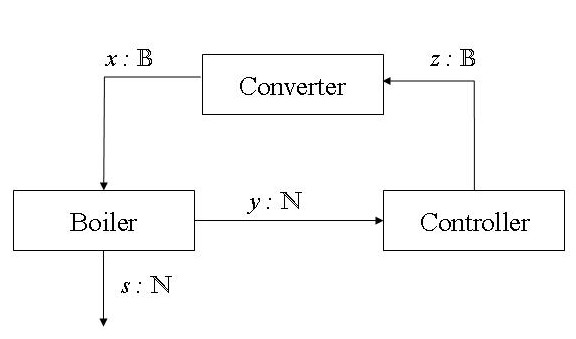
\includegraphics[width=7cm]{fig/BoilerSystemArch.jpg}
\end{spec}
}

The  \emph{SteamBoiler}  component works in time-synchronous manner: 
the current water level is controlled every time interval.
The boiler has two output channels with equal streams ($y = s$) and it
 fixes the initial water level to be $500$ gallons.
For every point of time the following must be true: if the pump is off, 
the boiler consumes at most $10$ gallons of water, 
otherwise (the pump is on) at most $10$ gallons of water will be added to its water tank.

The  \emph{Converter}   component converts the asynchronous output produced by the controller
to time-synchronous input for the steam boiler. 
Initially the pump is off, 
and at every later point of time (from receiving the first instruction 
from the controller) the output will be the last input from the controller. 

The   \emph{Controller}  component, 
contrary to the steam boiler component, 
 behaves in a purely asynchronous manner to keep
the number of control signals small, it means it might not be
desirable to switch the pump on and off more often than necessary.
The controller is responsible for
switching the steam boiler pump on and off. 
% 
If the pump is off: 
if the current water level is above $300$ gallons 
the pump stays off, otherwise the pump is started 
and will run until the water level reaches $700$ gallons. 
% 
If the pump is on: if the current water level is below $700$ gallons 
the pump stays on, otherwise the pump is turned off 
and will be off until the water level reaches $300$ gallons.

To show that the specified system fulfills the requirements we need to show that
the specification \emph{ControlSystemArch} is a refinement of the specification \emph{ControlSystem}. 
It follows from the definition of behavioral refinement that in order to verify that 
$
ControlSystem~ \leadsto ~ ControlSystemArch
$
it is enough to prove that
$$
\tlangle ControlSystemArch\trangle~ \Rightarrow ~\tlangle ControlSystem\trangle
$$
% 
Therefore, we have to  prove a \emph{lemma} 
that says the specification \emph{ControlSystemArch} is a refinement of the specification \emph{ControlSystem}:\\


\begin{isabellebody}%
\isacommand{lemma}\isamarkupfalse%
\ L{\isadigit{0}}{\isacharunderscore}ControlSystem{\isacharcolon} 
{\isasymlbrakk}\ ControlSystemArch\ s{\isasymrbrakk}\ {\isasymLongrightarrow}\ ControlSystem\ s\\
\end{isabellebody}% 


%==================================================

\subsection{Case Study 2: FlexRay Communication Protocol}

In this section we present a case study on FlexRay, 
communication protocol for safety-critical real-time applications. 
This protocol has been developed by the \fr Consortium \cite{FlexRayConsortium} 
for embedded systems in vehicles, and its advantages  
are deterministic real-time message transmission, fault tolerance, 
integrated functionality for clock synchronisation and higher bandwidth.

\fr contains a set of complex algorithms to provide the communication
services. From the view of the software layers above \fr only a few 
of these properties become visible. The most important ones are static 
cyclic communication schedules and system-wide synchronous clocks. 
These provide a suitable platform for distributed control algorithms 
as used e.g.\ in drive-by-wire applications. The formalization described 
here is based on the ``Protocol Specification 2.0''\cite{FlexRayProt}.
 
The static message transmission model of \fr is based
on \textit{rounds}. \fr rounds consist of a constant number of
time slices of the same length, so called \emph{slots}.
A node can broadcast its messages to other nodes at
statically defined slots. At most one node can
do it during any slot.

For the formalisation of \fr in \Focus we would like to refer to  \cite{efts_book} and \cite{spichkova}. 
To reduce the complexity of the system several aspects of \fr have been abstracted in this formalisation:
%
\begin{itemize}
\item[(1)] There is no clock synchronization or start-up phase since clocks are assumed to be synchronous. 
This corresponds very well with the \emph{time-synchronous} notion of \Focus.
%
\item[(2)] The model does not contain bus guardians that protect channels on the physical layer from interference caused by communication that is not aligned with FlexRay schedules.
%
\item[(3)] Only the static segment of the communication cycle has been included not the dynamic, 
as we are mainly interested in time-triggered systems.
%
\item[(4)] The time-basis for the system is one slot i.e.\ one slot \fr corresponds to one tick in in the formalisation.
%
\item[(5)] The system contains only one \fr channel. Adding a second channel 
would mean simply doubling the \fr component with a different configuration 
and adding extra channels for the access to the \emph{CNI\_Buffer} component.
\end{itemize}
% 
The system architecture consists of the following components, 
which describe the \fr components accordingly to the \fr standard~\cite{FlexRayProt}: 
%
\begin{itemize*}
	\item \emph{FlexRay} (general requirements specification), 
	\item \emph{FlexRayArch} (system architecture),   
	\item \emph{FlexRayArchitecture} 
(guarantee part of the system architecture), 
  \item \emph{Cable}, 
  \item \emph{Controller}, 
  \item \emph{Scheduler}, and 
  \item \emph{BusInterface}. 
  \end{itemize*}
  % 
We present the following \isah theories in this case study:
%
\begin{itemize*}
  \item \ist{FR\_types.thy} -- datatype definitions, 
	\item \ist{FR.thy} --  specifications of the system components and auxiliary functions and predicates, 
	\item \ist{FR\_proof} --   proof of refinement relation between the requirements and the architecture specifications.
\end{itemize*}
%
The type \emph{Frame} that describes a \fr frame 
 consists of a slot identifier of type \Nat~and the payload.
The type of payload is defined as a finite list of type \emph{Message}.
  The type \emph{Config} represents the bus configuration and contains the 
scheduling table \emph{schedule} of a node and the length 
of the communication round \emph{cycleLength}. 
A scheduling table of a node consists of a number of slots 
in which this node should be sending a frame with the corresponding identifier
(identifier that is equal to the slot).
%
\[
\begin{array}{lcl}
	\ntype Message & = & msg~(message\_id: \Nat, ftcdata : Data) \\
	\ntype Frame  & = & frm~(slot : \Nat, data : Data) \\
	\ntype Config & = & conf~(schedule: \nfst{\Nat}, cycleLength: \Nat )
\end{array}
\]
%
We do not specify the type \emph{Data} here to have a polymorphic specification 
of \fr (this type can be underspecified later to any datatype), therefore, in \isah it will be also defined as a polymorphic type \ist{$'$a}. 
The types \ist{$'$a~nFrame}, \ist{nNat} and \ist{nConfig} 
are used to represent sheaves of channels of types 
\emph{Frame}, \Nat~and \emph{Config} respectively.
In the specification group will be used 
channels \emph{recv} and \emph{activations}, as well as sheaves of channels 
(\emph{return$_1$, \dots,return$_n$}), ($c_1, \dots, c_n$), 
(\emph{store}$_1$, \dots, \emph{store}$_n$), (\emph{get}$_1$, \dots, \emph{get}$_n$), and 
(\emph{send}$_1$, \dots, \emph{send}$_n$).
We also need to declare some constant, \ist{sN}, for the number of specification replication and the corresponding number of channels in sheaves, as well as to define the list of sheaf upper 
bounds, \ist{sheafNumbers}.

The architecture of the \fr communication protocol  is specified
as the \Focus specification \emph{FlexRayArch}. 
Its assumption-part consists of three constraints:
(i) all bus configurations have disjoint scheduling tables, 
(ii) all bus configurations have the equal length of the communication round,
(iii) each \fr controller can receive tab most one data frame each time interval from the environment' of the \fr system.
The guarantee-part of \emph{FlexRayArch} is represented by the specification 
\emph{FlexRayArchitecture} (see below).  
  
{\footnotesize
\begin{spec}{\spc{FlexRayArch} \fconsts}{td}
\InOut{return_1 ,..., return_n : Frame}{store_1 ,..., store_n : Frame ;	get_1 ,..., get_n : \Nat}
\begin{array}{ll}
\uasm 
 &\forall i \in [1..n]: \msg{1}{return_i}\\
 &	DisjointSchedules(c_1 ,\dots, c_n)\\
 & IdenticCycleLength(c_1 ,\dots, c_n) \\
\ugar
 & (store_1 ,\dots, store_n, get_1 ,\dots, get_n) := \\
 & ~~~~~~FlexRayArchitecture(c_1 ,\dots, c_n)(return_1 ,dots, return_n)
\end{array}
\end{spec}
}


{\footnotesize
\begin{spec}{\spc{FlexRayArchitecture}\fconsts}{gb}
\centering
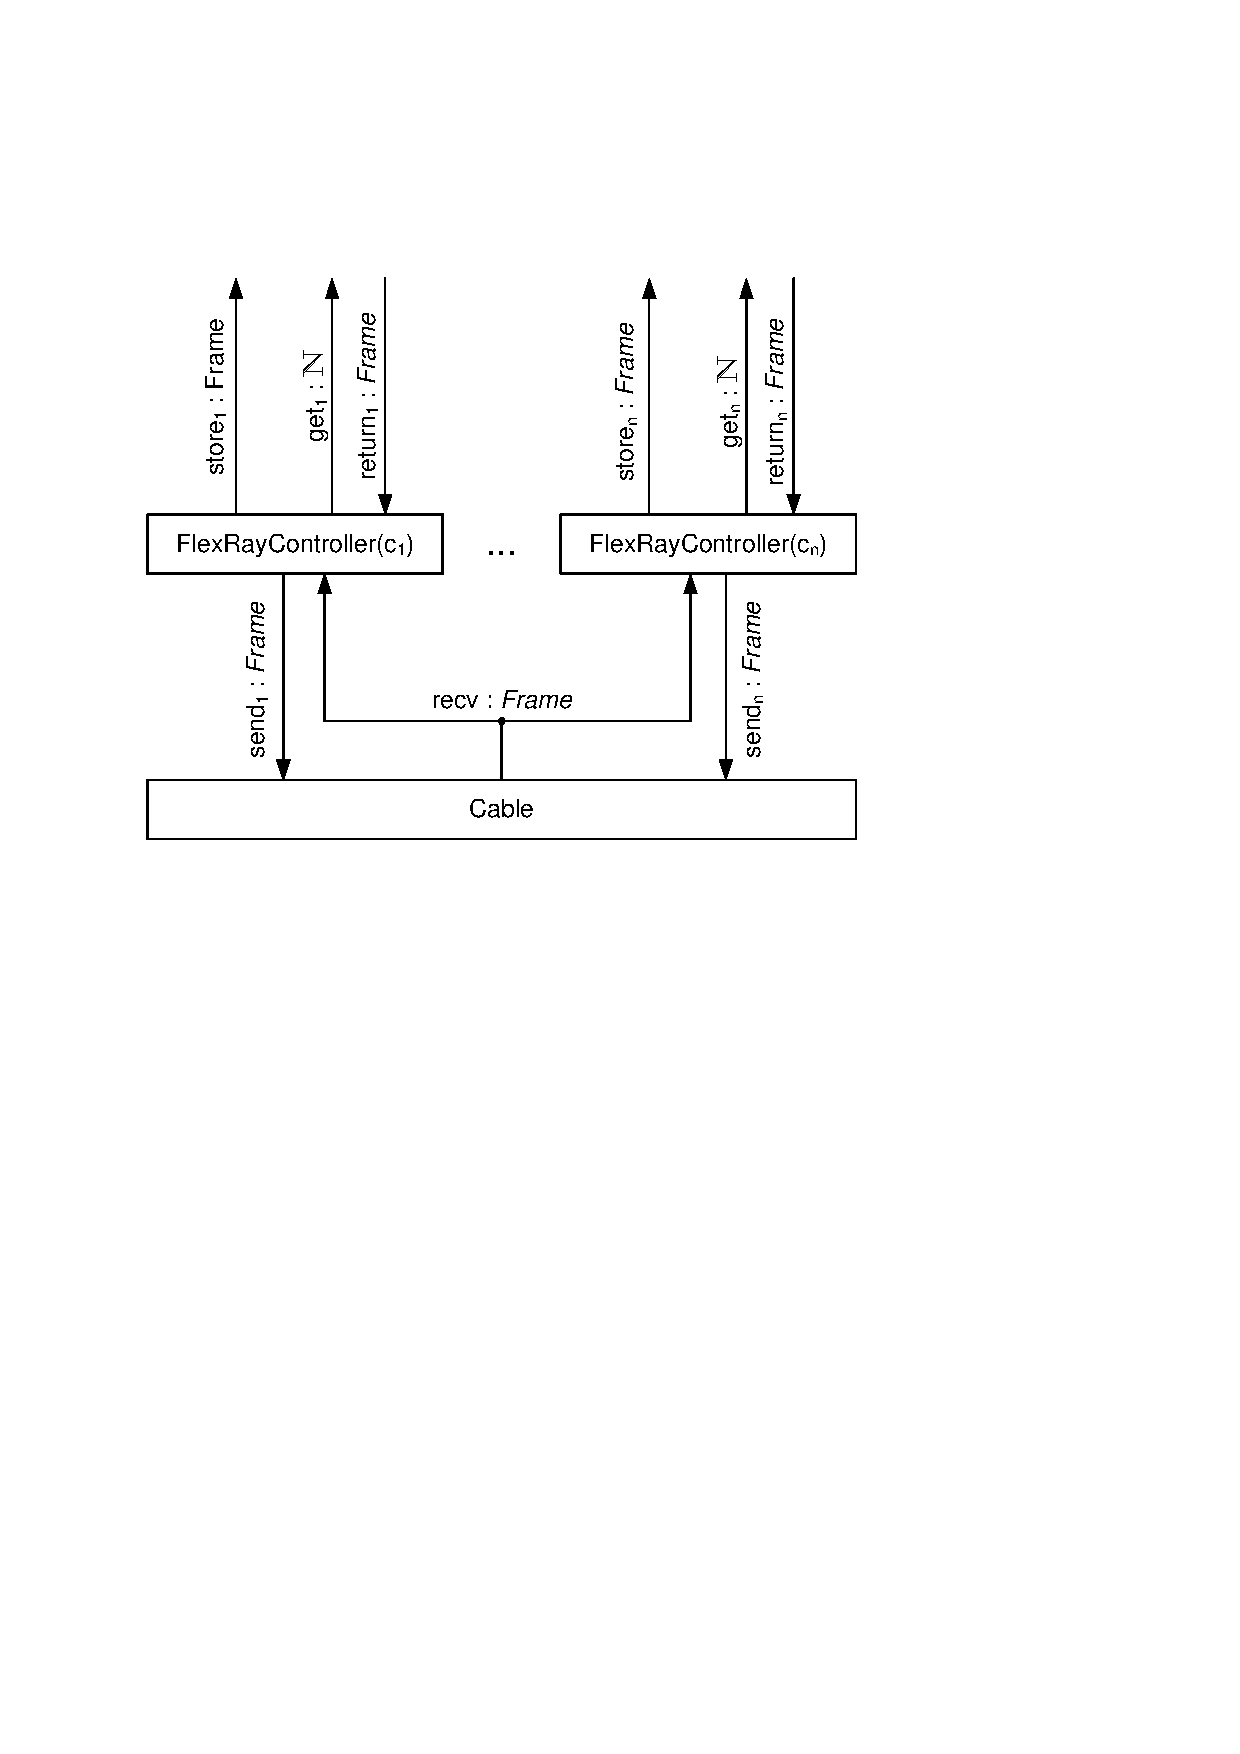
\includegraphics[width=8cm]{fig/flexray.pdf}
\end{spec}
}

\noindent
The component \emph{Cable} simulate the broadcast properties of the 
physical network cable -- 
every received \fr frame is resent to all connected nodes. 
Thus, if one \emph{FlexRayController} send some frame, 
this frame will be resent to all nodes 
(to all \emph{FlexRayController}s of the system).
The assumption is that all input streams of the component \emph{Cable} 
 are disjoint -- this holds by the properties of the 
\emph{FlexRayController} components and the overall system assumption that 
the scheduling tables of all nodes are disjoint.  
The guarantee is specified by the predicate \emph{Broadcast}. 

The \Focus specification \emph{FlexRayController} represent the controller component 
for a single node of the system. It consists of the components \emph{Scheduler} 
and \emph{BusInterface}. 
The \emph{Scheduler} signals the \emph{BusInterface}, that is responsible for 
the interaction with other nodes of the system (i.e. for the real send and receive of frames),  
on which time which \fr frames must be send from the node. 
The \emph{Scheduler} describes the communication scheduler. 
It sends at every time $t$ interval, which is equal modulo the length 
of the communication cycle to some \fr frame identifier (that corresponds to the number of the slot in the communication round) from the scheduler table, 
this frame identifier.  

%
The  specification \emph{FlexRay}  represents requirements on the protocol: 
If the scheduling tables are correct in terms of the predicates 
\emph{Disjoint\-Schedules} (all bus configurations have disjoint scheduling tables) 
and \emph{Identic\-Cycle\-Length} (all bus configurations have the equal length of the communication round), and 
also the \fr component receives in every time interval at most one message from each node 
(via channels $return_i$, $1 \le i \le n$), then
\begin{itemize}
	\item 
	the frame transmission by \fr must be correct in terms of the predicate 
	\emph{FrameTransmission}: if the time $t$ is equal modulo the length of the cycle (\fr communication round) 
to the element of the scheduler table of the node $k$, then this and only this node 
can send a data atn the $t$th time interval;
	\item 
	\fr component sends in every time interval at most one message to each node 
 via channels $get_i$ and $store_i$, $1 \le i \le n$).
\end{itemize}
%
To show that the specified system fulfill the requirements we need to show that
the specification \emph{FlexRayArch} is a refinement of the specification \emph{FlexRay}. 
It follows from the definition of behavioral refinement that in order to verify that 
$
FlexRay~ \leadsto ~ FlexRayArch
$
%
it is enough to prove that
$$
\tlangle FlexRayArch\trangle~ \Rightarrow ~\tlangle FlexRay\trangle
$$
% 
Therefore, we have to define and to prove a lemma, that says the specification 
\emph{FlexRayArch} is a refinement of the specification \emph{FlexRay}:
\\

\begin{isabellebody}%
\isacommand{lemma}\isamarkupfalse%
\ main{\isacharunderscore}fr{\isacharunderscore}refinement{\isacharcolon}\isanewline
FlexRayArch\ n\ nReturn\ nC\ nStore\ nGet\ %\isanewline
%\ \ 
{\isasymLongrightarrow}\ FlexRay\ n\ nReturn\ nC\ nStore\ nGet\isanewline
\end{isabellebody}%





%==================================================

\subsection{Case Study 3: Automotive-Gateway}


This section introduces the case study on telematics 
(electronic data transmission) gateway that was done for the 
Verisoft project\footnote{\url{http://www.verisoft.de}}. 
If the gateway receives from a ECall application of a vehicle
a signal about crash 
(more precise, the command to initiate the call to the Emergency Service Center, ESC), 
and after the establishing the connection it receives 
 the command to send the crash data, received from sensors.
These data are restored 
 in the internal buffer of the gateway  and should  
 be resent to the ESC and 
 the voice communication will be established, assuming that
	there is no connection fails.  
The system description consists of the following specifications: 
\begin{itemize*}
	\item \emph{GatewaySystem} (gateway system architecture), 
	\item \emph{GatewaySystemReq} (gateway system requirements), 
	\item \emph{ServiceCenter} (Emergency Service Center),
	\item \emph{Gateway} (gateway architecture), 
	\item \emph{GatewayReq} (gateway requirements),
	\item \emph{Sample} (the main  component describing its logic), 
	\item \emph{Delay} (the  component   modelling the communication delay), and
	\item \emph{Loss} (the  component modelling the communication loss).  
\end{itemize*}
%  
We present the following \isah theories in this case study:
\begin{itemize*}
  \item \ist{Gateway\_types.thy} --  datatype definitions, 
	\item \ist{Gateway.thy} --  specifications of the system components, 
	\item \ist{Gateway\_proof} --  proofs of refinement relations between the requirements and the architecture specifications (for the components \emph{Gateway} and \emph{GatewaySystem}).
\end{itemize*}
%
The datatype \emph{ECall\_Info} represents a tuple, 
consisting of the data that the Emergency Service Center needs -- here we specify these data to contain the vehicle coordinates and the collision speed, they can also extend by some other information.  
The datatype \emph{GatewayStatus} represents the status (internal state) of the gateway.
%
\[
\begin{array}{lcl}
  \ntype Coordinates &=& \Nat \times \Nat
  \\
  \ntype CollisionSpeed &=& \Nat
  \\
	\ntype ECall\_Info &=& ecall(coord \in Coordinates, speed \in CollisionSpeed)
	\\
	\ntype GatewayStatus &=& 
	\{~ init\_state,~ call,~ connection\_ok,\\
	&& ~ ~sending\_data,~ voice\_com ~\}
\end{array}
\]
To specify the automotive gateway we will use a number of datatypes 
consisting of one or two elements: 
$\{init, send\}$, $\{stop\_vc\}$, $\{vc\_com\}$ and $\{sc\_ack\}$. 
We name these types \emph{reqType}, \emph{stopType}, \emph{vcType} and \emph{aType} correspondingly.

The \Focus specification of the general gateway system architecture is presented below:

\begin{spec}{\spc{GatewaySystem}(\nconst d \in \Nat)}{gb}
\centering 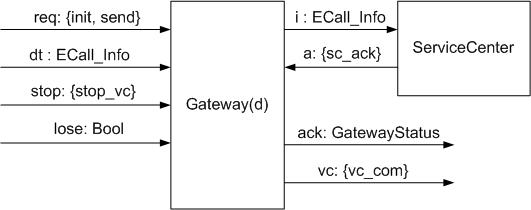
\includegraphics[width=7cm]{fig/gatewaySystem.jpg}
\end{spec} 

\noindent
The stream \emph{loss} is specified to be a time-synchronous one (exactly one message each time interval). 
It represents the connection status: 
the message \ntrue~at the time interval $t$ corresponds to the connection 
failure at this time interval, the message \nfalse~at the time interval $t$ means that 
at this time interval no data loss on the gateway connection.

The specification \emph{GatewaySystemReq} specifies the requirements for the component \emph{GatewaySystem}:
Assuming that the input streams \emph{req} and \emph{stop} can contain at every time interval at most one message, and assuming that the stream \emph{lose} contains at every time interval exactly one message. 
If 
\begin{itemize*}
	\item 
	at any time interval $t$ the gateway system is in the initial state, 
	\item
	at time interval $t+1$ the signal about crash comes at first time 
	(more precise, the command to initiate the call to the ESC,
	\item 
	after $3+m$ time intervals the command to send the crash data comes at first time,
	\item 
	the gateway system has received until the time interval $t+2$ the crash data,  
	\item 
	there is no connection fails from the time interval $t$ until the time interval $t + 4 + k + 2d$,
	\end{itemize*}
%
then at time interval $t + 4 + k + 2d$ the voice communication is established.


The component \emph{ServiceCenter} represents the interface behaviour of the ESC 
(wrt. connection to the gateway): 
if at time $t$ a message about a vehicle crash comes, it acknowledges this event by sending 
the at time $t+1$ message \emph{sc\_ack} that represents the 
attempt to establish the voice communication with the driver or a passenger of the vehicle. 
if there is no connection failure, after $d$ time intervals the voice communication will be started. 

We specify the gateway requirements (\emph{GatewayReq}) as follows: 
	\begin{enumerate}
	\item 
	%1
	If at time $t$ the gateway is in the initial state $init\_state$, and it gets 
	the command to establish the connection with the central station, and also there is no 
	environment connection problems during the next 2 time intervals, 
	it establishes the connection at the time interval $t+2$. 
	\item 
	%2
	If at time $t$  the gateway has establish the connection, 
	and it gets the command to send the ECall data to the central station, and also there is no 
	environment connection problems during the next $d+1$ time intervals, 
	then it sends the last corresponding data. 
        The central station becomes these date at the time $t+d$.
	% 
	\item 
	%3
	If the gateway becomes the acknowledgment from the central station 
	that it has receives the sent ECall data, and also there is no 
	environment connection problems, then the voice communication is started.
  \end{enumerate}
 %
 The specification of the gateway architecture, \emph{Gateway}, is parameterised one: 
the parameter $d \in \Nat$ denotes the communication delay 
between the central station and a vehicle. 
This component consists of three subcomponents: \emph{Sample}, \emph{Delay}, 
and \emph{Loss}: 
 
\begin{spec}{\spc{Gateway}(\nconst d \in \Nat)}{td}
\centering 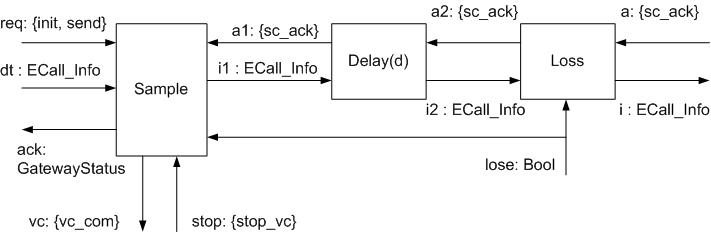
\includegraphics[width=10cm]{fig/gateway.jpg}
\end{spec} 
  
\noindent
The component \emph{Delay} models the communication delay. 
Its specification is parameterised one: 
it inherits the parameter of the component \emph{Gateway}. 
This component simply delays all input messages on $d$ time intervals. 
During the first $d$ time intervals no output message will be produced. 

The component \emph{Loss} models the communication loss between 
the central station and the vehicle gateway: 
if during time interval $t$ from the component \emph{Loss} no message about a 
lost connection comes, the messages come during time interval 
$t$ via the input channels $a$ and $i2$ will be forwarded without any delay via channels 
$a2$ and $i$ respectively. 
Otherwise all messages come during time interval 
$t$ will be lost.  
  
The component \emph{Sample} represents the logic of the gateway component. 
If it receives from a ECall application of a vehicle 
 the command to initiate the call to the ESC it tries 
 to establish the connection.
If the connection is established, and the component \emph{Sample} receives 
from a ECall application of a vehicle
 the command to send the crash data, which were already received and stored 
 in the internal buffer of the gateway, 
 these data will be resent to the ESC. 
 After that this component waits to the acknowledgment from the ESC. 
 If the acknowledgment is received, the voice communication will be established, assuming that
	there is no connection fails.

For the component \emph{Sample} we have the assumption, that the 
streams $req$, $a1$, and $stop$ can contain at every time interval at most one message, 
and also that the stream $loss$ must contain at every time interval exactly one message. 
This component uses local variables \emph{st} and \emph{buffer} (more precisely, 
a local variable \emph{buffer} and a state variable \emph{st}). 
The guarantee part of  the component \emph{Sample} can be specified as a timed state transition diagram  (TSTS) 
and an expression which says how the local variable 
\emph{buffer} is computed, or using the corresponding table representation, which is semantically equivalent to the TSTD.  
  
  
 \begin{figure}[h]
	\begin{center}
		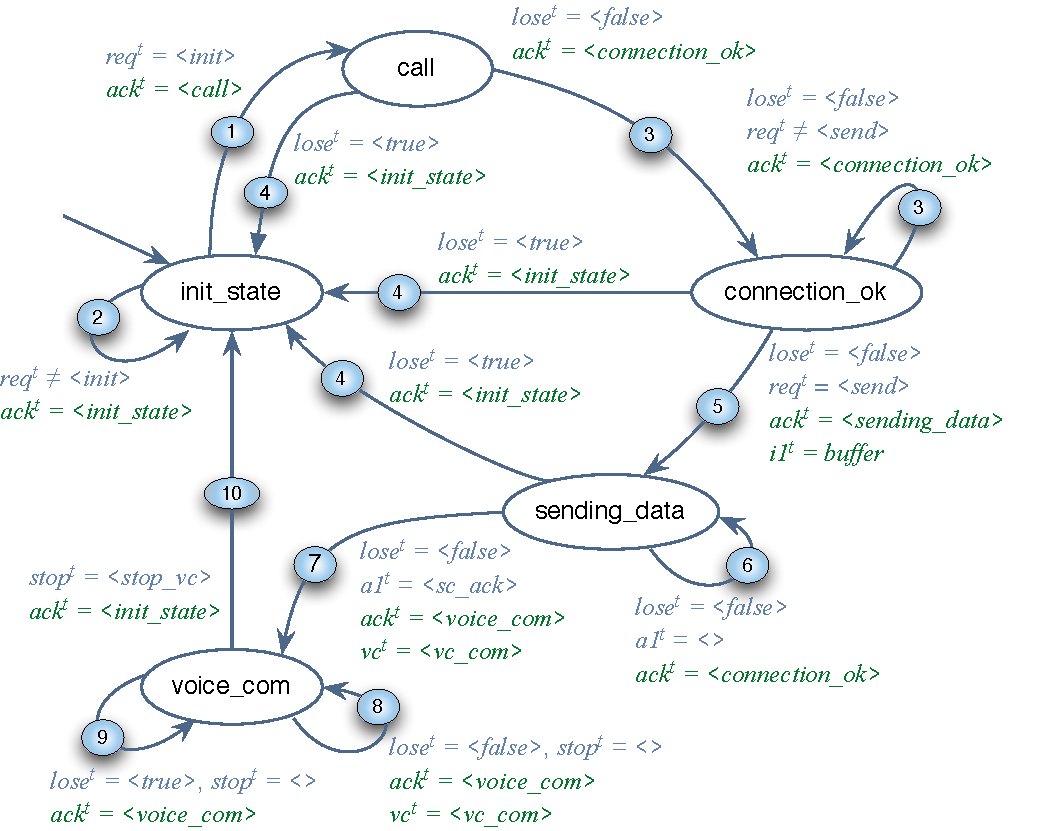
\includegraphics[scale=0.6]{fig/gatewayTSTD.pdf}
	\end{center}
	\caption{Timed state transition diagram for the component Sample}
	\label{fig:gateway_std}
\end{figure} 


  To show that the specified gateway architecture fulfils the requirements we need to show that
the specification \emph{Gateway} is a refinement of the specification \emph{GatewayReq}. 
Therefore, we need to define and to prove the following lemma:
\\

\begin{isabellebody}%
\isacommand{lemma}\isamarkupfalse%
\ Gateway{\isacharunderscore}L{\isadigit{0}}{\isacharcolon}\isanewline
\ Gateway\ req\ dt\ a\ stop\ lose\ d\ ack\ i\ vc\isanewline
\ {\isasymLongrightarrow} 
\ GatewayReq\ req\ dt\ a\ stop\ lose\ d\ ack\ i\ vc
\end{isabellebody}%

~\\
To show that the specified gateway architecture fulfills the requirements we need to show that
the specification \emph{GatewaySystem} is a refinement of the specification \emph{GatewaySystemReq}. 
Therefore, we need to define and to prove the following lemma:
\\

\begin{isabellebody}%
\isacommand{lemma}\isamarkupfalse%
\ GatewaySystem{\isacharunderscore}L{\isadigit{0}}{\isacharcolon}\isanewline
\ GatewaySystem\ req\ dt\ stop\ lose\ d\ ack\ vc\isanewline
\ {\isasymLongrightarrow} 
\ GatewaySystemReq\ req\ dt\ stop\ lose\ d\ ack\ vc\isanewline
\end{isabellebody}%  
  
%